\chapter{Lexical Substitution}
\label{ch:lexsub}

This chapter shows new model of lexical substitution, and related
material. The work in this chapter has been published in
\newcite{roller:2016:naacl}.

\section{Chapter Introduction}

%We discuss the Lexical Substitution task, in which the word meaning in context
%is described or evaluated, not through dictionary senses, but through
%substitutes or paraphrases suggested by annotators
%\cite{mccarthy:2007:semeval}. We review various approaches to the task, and
%focus on one particularly simple, modern method which performs competitively to
%State of the Art \cite{melamud:2015:vsm}. We describe the intuitions of this
%model, and propose Probability-in-Context, a variation on this simple idea. We
%find our proposed model significantly outperforms baselines, and analyze why it
%improves over the prior work.

Our discussions in the previous chapters assumed that a word has only one
meaning, and that this meaning does not change with respect to context.
However, some lexical entailments may hold in particular contexts but not
in others. In this chapter, we consider the task of {\em Lexical Substitution},
where we must propose paraphrases for a given target word appearing in
a particular context. We propose Probability in Context (PIC), an unsupervised
measure for estimating a paraphrase's appropriateness for a given target and
context. We show our measure outperforms baseline measures, especially in an
experimental setup where paraphrases are considered from the entire vocabulary.

\section{Lexical Substitution}

In our discussion of lexical relationships in the previous two chapters, we
assumed that words are {\em monosemous}, or that they have only one meaning.
However, words like \lit{bright} have multiple meanings, which change depending
on context, as in \lit{bright girl} and \lit{bright coat}. When a word has
multiple meanings, it is {\em polysemous}, and polysemy is yet another source
of ambiguity in natural language.

It is still unclear what representation should even be chosen
to represent polysemous words. One option is the use of a lexicon, like the
dictionary.  Lexicographers are responsible for cataloging and defining word
senses; one may see this in the multiple definitions provided by the Oxford
English Dictionary or Merriam Webster, but even professional lexicographers
often disagree on how many senses a word has. For example, \lit{bank} has
three noun senses in Webster's dictionary, but only two in Oxford's.
WordNet \cite{miller:1995:acm} is one of the most popular and heavily used
computational dictionaries, and is notoriously fine-grained (it gives 10
noun senses for \lit{bank}).

Even after one fixes the inventory of word senses, labeling a particular
instance of a word with its sense is fraught with its own difficulties:
non-experts have very low inter annotator agreements \cite{yong:1999:siglex},
and even lexicographers will disagree often \cite{kilgarriff:2000:ch}.
Results in computational approaches to Word Sense Induction (WSI) and Word
Sense Disambiguation (WSD) reflect this task difficulty \cite{mccarthy:2009:llc,navigli:2009:csur}.

Distributional Semantics offers an alluring alternative path, given its ability
to measure the {\em graded} levels of similarity between words
\cite{erk:2008:emnlp}.  One possibility to represent each of a word's senses
using a separate vector, resulting in multiple vectors per word
\cite{reisinger:2010:naacl,huang:2012:acl}, and then use
these prototypes appropriately in downstream tasks. If one takes this idea to
its absolute extreme, one can imagine a new vector for every instantiation of a
word. In this extreme, one may choose not to create a unique vector for every
word, but instead model how meaning {\em shifts} in a particular given context
\cite{erk:2008:emnlp,erk:2010:gems}.

One way to measure this has been the Lexical Substitution task. In
the Lexical Substitution task, we are provided with a sentential context, and
must suggest {\em substitutes} which can replace the given target word, while
preserving the meaning of the entire sentence
\cite{mccarthy:2007:semeval,biemann:2012:lrec,kremer:2014:eacl}. For
example, when provided the sentence
\begin{quote}
  \lit{The \target{bright} scientist reads the paper,}
\end{quote}
annotators will readily offer substitutes like the \lit{clever scientist} or
\lit{smart scientist}. Similarly, when provided the sentence
\begin{quote}
  \lit{The girl put on her \target{bright} coat,}
\end{quote}
humans will suggest the \lit{colorful coat} instead. However, annotators
may also choose creative or nonstandard suggestions, especially when provided
excerpts from fiction. In one dataset, humans provided with the context
\begin{quote}
  \lit{Tara stood stock-still, waiting for the first tiny gleam from the
  scout craft to appear in the darkness of the \target{wormhole},}
\end{quote}
human annotators considered {\em portal} and {\em rift} to be excellent
substitutes. These substitutes take into account the Science Fiction context of
the sentence, indicating the task is more complicated than simple synonymy.
Indeed, in one one lexical substitution dataset, only 9\% of substitutes in
their dataset were direct synonyms in WordNet \cite{kremer:2014:eacl}.

\section{Prior Work}

The original SemEval shared task released a moderately sized dataset and
defined the task \cite{mccarthy:2007:semeval}. The experimental setup was
specifically designed in order to elicit responses to polysemy in human
annotators. The corpus collectors selected a set of 2211 sentences containing
a targeted list polysemous words curated both manually and automatically using
lexical resources. These words cover several part-of-speech tags, and sentences
were manually selected to prevent primary senses from dominating the corpus.
Five human annotators were then asked to propose substitutes for the target
words in the sentential context: phrases and moderate generalizations were
allowed, but discouraged. The unification of substitutions resulted in a ranked
list of substitutes for every sentential context. Shared task participants
were asked to perform the same task computationally: both suggesting and
ranking possible substitutes.

Performance for the task was measured in {\em precision out of ten} (oot),
where a system was able to make up to ten guesses and the average percentage
of correct guesses across all sentences was reported; and {\em best}, where
a system provided its single best substitute and evaluated on whether that
substitute was proposed by any annotator.

A clear majority of systems used some lexical resource, like WordNet, to first
provide a list of possible substitutions, and then filtered or ranked that list
using their own research methods. Several used a mixture of co-occurrences or
$n$-grams to find good matches, and several used distributional methods to rank
the substitutes, almost no systems used existing WSD datasets
\cite{mccarthy:2007:semeval}. The strongest team on the {\em best} metric used a
supervised approach where substitutes were ranked
using features like $n$-gram likelihood \cite{yuret:2007:semeval}, while
the strongest performing system in the {\em oot} metric accidentally exploited
a flaw in the evaluation by proposing the same substitute many times
\cite{giuliano:2007:semeval}. The
literature has since varied substantially on experimental setup and evaluation
metrics. Nonetheless, the task provided an interesting test bed for a
variety approaches, including distributional approaches, language modeling
approaches, and some supervised approaches \cite{szarvas:2013:naacl}.

\subsection{Unsupervised approaches}

One major insight from the competition was the importance of syntagmatic fit in
lexical substitution with the success of $n$-gram based models.
\newcite{erk:2008:emnlp} proposed a model for offering each unique word
occurrence its own individualized word vector, allowing polysemy to be modeled
without explicit word senses, and applied these sense-free representations
to the task of lexical substitution. Their representations modified the
out-of-context word vectors by averaging it with other possible fillers for
the same contexts.
For example, in \lit{the fielder {\em catches}}, they would consider
verbs which take \lit{fielder} in the subject position. Since their
work focused more on innovations in representations of polysemy, they
evaluated their system on its ability to identify correct substitutes from
a candidate list, and did not consider its ability to {\em generate} substitutes
from the entire vocabulary.

\newcite{thater:2009:ati,thater:2010:acl} expanded on the this idea of inverse
selection preferences by proposing a {\em second-order} distributional space,
where syntactic co-occurrences were modeled via a sparse tensor representation
similar to TypeDM \cite{baroni:2011:gems}, and using multiple folds over the
tensor to produce a unique vector for each word in context.
\newcite{thater:2011:ijcnlp} refine and simplify on this second-order view of
the previous models by proposing to re-weight a word's syntactic co-occurrences
based on their similarity to the present context.
This unsupervised method remained one of strongest performing systems even when
applied to new datasets \cite{kremer:2014:eacl} and compared to some
supervised systems. Along a similar path, \newcite{melamud:2015:naacl} proposed
an alternative second order model based on using Google's web corpus of
5-grams.

\newcite{dinu:2010:emnlp} showed that latent-factor distributional models like
Latent Dirichlet Allocation \cite{blei:2003:jmlr} could allow for evaluating
the particular fit of a given substitute. They considered two latent
factorization models (LDA and NNMF) and showed that context could successfully
modulate over varying latent senses of a particular word in a bag-of-words
context. This insight in the power of low-rank factorizations later turns
out to be valuable in later lines of work
\cite{melamud:2015:vsm,roller:2016:naacl}. We defer discussion of these works
until Section~\ref{sec:melamud}, due to their central role in this chapter.

\newcite{vandecruys:2011:emnlp} observed that syntax-based distributional
models tend to provide the strongest results, yet individual examples in
lexical substitution data {\em should} require a wider understanding of the
context, like in the \lit{wormhole} example provided earlier. They proposed a
{\em joint} latent factorization model over both a wide bag-of-words
co-occurrences with the functional, syntactic context. Although this line of
work has not seen a large degree of follow up, the author of this dissertation
hopes future research will reconsider this path.

More recently, some research has used neural language models for the task
of lexical substitution. \newcite{kawakami:2016:iclr} propose using word
alignments from translation tasks in order to identify the different senses of
a word in the hidden state of a bidirectional RNN. The intuition is that two
tokens which translate into the same foreign token have the same underlying
sense, while two tokens which translate into different foreign tokens must
represent a polysemous term, an idea has a long history in the literature
\cite{resnik:1999:nle,diab:2003:phd,bannard:2005:acl}. Since their model
requires substantial aligned translation corpora, it is not directly comparable
to the other models exploring the task. \newcite{melamud:2016:conll}
applied the same neural architecture, trained in an English-only language
modeling task, but found it did not achieve state-of-the-art performance.

\subsection{Supervised approaches}

Another vein of research has treated Lexical Substitution as a truly
supervised research problem, as opposed to the predominantly unsupervised or
knowledge-transfer approaches listed above. For example, the original SemEval
task tuned a threshold on likelihoods obtained from a language
model \cite{yuret:2007:semeval}. Others have proposed more sophisticated
architectures based on producing context features for the target token
\cite{biemann:2012:lrec}, or a fully delexicalized classifier which learns over
features extracted via a (target, substitute) pair \cite{szarvas:2013:naacl}.
Another approach from \newcite{szarvas:2013:emnlp} notes that previous
approaches emphasize the importance of ranking properly, and proposes to treat
lexical substitution as a true ranking problem. This substantially outperforms
the other ranking approaches, but the comparison is unfair due to differing
levels of supervision.

\section{Context Vectors for LexSub (Melamud et al. 2015b)}
\label{sec:melamud}

We now consider the unsupervised models of \newcite{melamud:2015:vsm}, which
are central to the contributions of our own work.
\newcite{melamud:2015:vsm} introduce a simple, but high-performing method,
based on the Syntactic Skip-Gram Negative Sampling model of
\newcite{levy:2014:acl}. As with other unsupervised models, it combines a
measure of an out-of-context substitute's suitability, with a special
in-context appropriateness measure \cite{erk:2008:emnlp}. Unlike the many of
the previous unsupervised models, it does not rely on computing large
second-order vectors, and can in fact be used with off-the-shelf syntactic
word2vec vectors.

As emphasized in Chapters \ref{ch:background} and \ref{ch:hpm}, when creating
low dimensional vectors, a high-dimensional co-occurrence matrix $\mM$ is
factorized or approximated with two lower-rank matrices \cite{levy:2014:nips}:
\begin{equation*}
  \mM = \mV\mC\trans,
  \tag{\ref{eqn:factorization} revisited}
\end{equation*}
where $\mV$ is the matrix of word vectors, and $\mC$ is the matrix of
{\em context vectors}. The primary insight of \newcite{melamud:2015:vsm}
was that these context vectors can be used to evaluate the suitability of a
novel substitute in a particular given context.

Suppose we have sentence like \lit{The very \target{bright} girl reads}, and we
want to evaluate which is a better substitute: \lit{smart} or \lit{colorful}.
If we were to extract the syntactic contexts of the target \lit{bright}, as in
the previous chapter, we would end up with exactly two contexts:
\ctx{advmod:very}, indicating our target is modified by \lit{very}, and
\ctx{amod\depinv:girl}, indicating that our target modifies
\lit{girl}. We may then use the context matrix $\mC$ to look up the
vectors for these two contexts, and judge their similarity to the possible
substitutes.

Figure~\ref{fig:substitution} provides an intuitive illustration of the idea:
by looking at the context vector \ctx{amod\depinv:girl}, we see that it is
closer to the substitute \lit{smart} than the substitute \lit{colorful}. The
context \ctx{advmod:very}, on the other hand, lies somewhere about halfway
between the two substitutes, indicating both substitutes are equally appropriate
for this context.

\begin{figure}
\centering
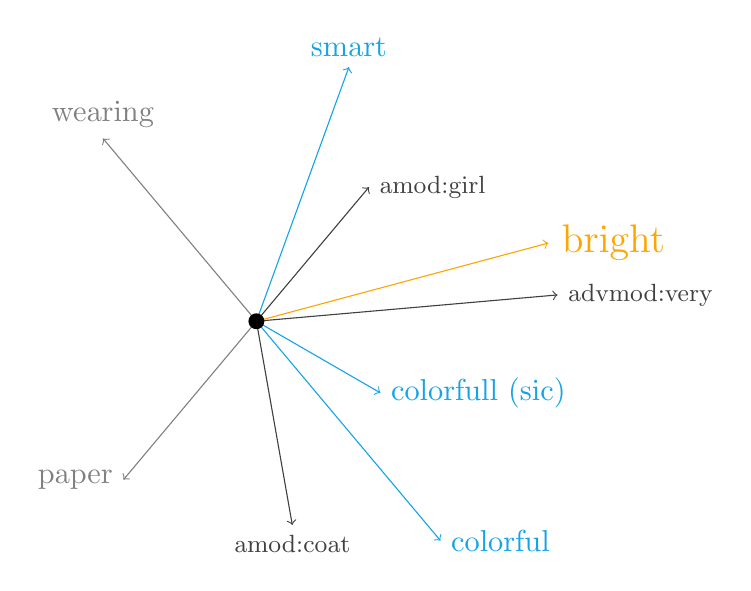
\begin{tikzpicture}[scale=\textwidth/6cm]
    \fontsize{11}{11}\selectfont
    \coordinate (origin) at (0,0);
    \draw [->,Gray] (origin) -- (130:1.5) node[above] {{wearing}};
    \draw [->,Gray] (origin) -- (230:1.3) node[left] {{paper}};
    \draw [->,Cerulean] (origin) -- (310:1.8) node[right] {{colorful}};
    \draw [->,Cerulean] (origin) -- (330:0.9) node[right] {{colorfull} (sic)};
    \draw [->,Cerulean] (origin) -- (70:1.7) node[above] {{smart}};
    \draw [->,darkgray] (origin) -- (5:1.9) node[right] {{\small \ctx{advmod:very}}};
    \draw [->,darkgray] (origin) -- (280:1.3) node[below] {{\small \ctx{amod\depinv:coat}}};
    \draw [->,darkgray] (origin) -- (50:1.1) node[right] {{\small \ctx{amod\depinv:girl}}};
    \fontsize{14}{14}\selectfont
    \draw [->,Orange] (origin) -- (15:1.9) node[right] {\target{bright}};
    \fill (origin) circle (0.05);
\end{tikzpicture}
\caption{Cartoon illustration of how context vectors can disambiguate word senses.}
\label{fig:substitution}
\end{figure}

Formally, for a given target $t$, substitute $s$ and context $C$, the final
{\addCos} score is defined as:
\begin{equation}
  \text{addCos}(\vs|\vt,C) = \text{cos}(\vs, \vt) + \sum_{c\in C} \text{cos}(\vs, \vc).
\end{equation}
Note that the equation has two components: the first measures the {\em
out-of-context} similarity between the target $t$ and the substitute $s$ using
basic cosine similarity. The second half of the measure encodes the {\em
in-context} appropriateness, by considering substitute with respect to
each of the syntactic contexts.

This formulation is considerably simpler than many of the other models
in the prior work, which require significant overhead for space creation
or re-weighting of terms, but performs competitively with even more recent
models. For this reason, it acts as a particular strong and standard baseline,
which can help calibrate work with different vocabulary or experimental
conditions.

\newcite{melamud:2015:vsm} also consider variants of this measure, including
{\em balAddCos}, which equally weights the out-of-context similarity with the
in-context appropriateness:
\begin{equation}
  \text{balAddCos}(s|t,C) = \text{cosine}(s, t) + \frac{1}{|C|}\sum_{c\in C} \text{cosine}(s, c).
\end{equation}
This alternative measure reweights the similarities obtained from the context
vectors so that the out-of-context similarity and in-context appropriateness
are given equal weight. The choice between the \addCos and \balAddCos is
an empirical one, and performance of either could vary across datasets or
evaluation metrics.

\section{Probability-in-Context (PIC)}

We propose an extension of the context vector measure of
\newcite{melamud:2015:vsm}, called Probability-in-Context (PIC).  We note that
our measure is {\em not} a well defined probability measure; rather the name was
simply chosen for the purpose of the paper's title.

Similar to \balAddCos, the measure has two equally-weighted, independent
components measuring the appropriateness of the substitute for both the target
and the context, each taking the form of a softmax:
\begin{equation}
  \begin{aligned}
  \mbox{PIC}(s | t, C) &= P(s | t) \times P(s | C)\\
  P(s | t) &= \frac{1}{Z_t}\exp\left\{\vs^\top \vt\right\}\\
  P(s | C) &= \frac{1}{Z_C}\exp\left\{\sum_{c\in C}\vs^\top\left[\mW\vc + \vb\right]\right\},
  \end{aligned}
  \label{eqn:pic}
\end{equation}
where the $t$ is the target word, $s$ is a proposed substitute, $C$ is the set
of syntactic contexts, and $Z_t$ and $Z_C$ are normalizing constants. Our
model differs from \mbox{\balAddCos} in two important ways. First, our
similarity measure uses {\em unnormalized} inner products $s^\top t$
and $s^\top c$, rather than {\em normalized} cosine similarities; and
second, we introduce two  free parameters, $W$ and $b$, which act as a linear
transformation over the original context vectors. These parameters are
estimated from the {\em original corpus}, and are trained to maximize the
prediction of a {\em target} from only its syntactic contexts. These parameters
are {\em not} trained on the lexical substitution dataset, and
therefore serve only to tune how the fixed distributional vectors act in this
alternative objective function.

Nonetheless, to identify the contribution of this parameterization versus the
softmax objective, we also introduce to a non-parameterized PIC ({\em nPIC}),
which does not contain the extra parameters:
\begin{equation}
  \begin{aligned}
  \mbox{nPIC}(s | t, C) &= P(s | t) \times P_n(s | C)\\
  P_n(s | C) &= \frac{1}{Z_n}\exp\left\{\sum_{c\in C}\vs^\top \vc\right\}
  \end{aligned}
  \label{eqn:npic}
\end{equation}

One may ask why not train or tune the embeddings to optimize this softmax
objective directly, rather than learning the parameterization which adjust the
embeddings? This ultimately is an empirical question, and our initial tests
found that training new embeddings from scratch did not result in stronger
performance. Additionally, the SGNS embeddings are already popular and
well-understood in relation to traditional distributional semantics.
Furthermore, we can re-use the embeddings of \newcite{melamud:2015:vsm} to
ensure that experimental conditions are fair to both models, and that
the quality of embeddings remains consistent across comparisons.


\section{Experiments}
We compare our proposed measures to three baselines: \ooc, the Out-of-Context
cosine similarity between the word and target $\mbox{cos}(s, t)$; and the
\mbox{\addCos} and \mbox{\balAddCos} measures.
We evaluate on three lexical substitution datasets:
\begin{itemize}
\item {\bf SE}: The dataset used in the original SemEval 2007 shared task
\cite{mccarthy:2007:semeval} consists of 201 words manually chosen to exhibit
polysemy, with 10 sentences per target. For a given target in a particular
context, five annotators were asked to propose up to 3 substitutes. As all our
experiments are unsupervised, we always evaluate over the entire dataset,
rather than the original held-out test set.
\item {\bf Coinco}: The Concepts-in-Context dataset \cite{kremer:2014:eacl} is a
large lexical substitution corpus with proposed substitutes for nearly all
content words in roughly 2,500 sentences from a mixture of genres (newswire,
emails, and fiction). Crowdsourcing was used to obtain a minimum of 6
contextually-appropriate substitutes for over 15k tokens. Unlike SemEval, this
dataset was not constructed specifically to capture polysemy; nonetheless,
many substitutes vary considerably for different sentential contexts,
indicating that polysemy is definitely present.
\item {\bf TSWI}: The Turk bootstrap Word Sense Inventory 2.0 \cite{biemann:2012:lrec}
is a crowdsourced lexical substitution corpus focused on about 1,000 common
English nouns. The dataset contains nearly 25,000 contextual uses of these
nouns. Though the dataset was originally constructed to induce a word-sense
lexicon based on common substitution patterns, here we only use it as a
lexical substitution dataset.
\end{itemize}

We compare models on two variations of the lexical substitution task: candidate
ranking and all-words ranking. In the {\em candidate ranking} task, the model
is given a list of candidates and must select which are most appropriate for
the given target. We follow prior work in pooling candidates from all
substitutions for a given lemma and POS over all contexts, and measure
performance using Generalized Average Precision (GAP) \cite{kishida:2005:gap}.
GAP is similar to Average Precision, but weighted by the number of times a
substitute was given by annotators. Intuitively, it measures the number of
"correct" points the model has obtained at every point, normalized by the
maximum number of possible points obtainable at that rank.  For a particular
target, suppose $h_1,\ldots,h_n$ are an ordered list of the model's scores
assigned for the possible substitutes, so that the substitute with the best
score comes first. Let's also assume that $g_1,\ldots,g_n$ is the sorted gold
list of scores, and that $g(h_i)$  gives the gold score of the
substitute predicted at $h_i$. GAP is then defined in terms of the precision
over all possible values of $i$:
\begin{align*}
  \text{GAP} & = \frac{1}{R}\sum_{k=1}^n\left[\sum_{i=1}^k\frac{g(h_i)}{i}\right]\\
  R & = \sum_{k=1}^n\left[\frac{1}{k}\sum_{i=1}^n g_i\right]
\end{align*}
Intuitively, GAP measures 1.0 when the model perfectly ranks the list, and 0.0
when the model provides the reverse listing. Partial credit is awarded for
providing items in roughly the correct order, weighted by how important the
items are in the gold scores.

Our second task is the much more difficult task of {\em all-words ranking}. In
this task, the model is not provided any gold list of candidates, but must
select possible substitutes from the entire vocabulary. All models are also
hardcoded not to predict substitutes with the same stem as the target, e.g. for
the \lit{bright girl} example, models cannot predict \lit{brighter} or
\lit{brightest}.
On this all-words ranking task, we evaluate performance with (micro) mean
Precision@1 and P@3: that is, of a system's top one/three guesses, the
percentage also given by human annotators.  These evaluation metrics are
similar to the {\em best} and {\em oot} metrics reported in the literature, but
we find P@1 and P@3 easier to interpret and analyze. In case annotators did
not provide three unique substitutes, that particular substitution is divided
by the total number of unique substitutions.

\subsection{Vectors and Training Procedure}

We use the word and context vectors released by \newcite{melamud:2015:vsm},
which were previously shown to perform strongly in lexical substitution tasks,
and to ensure our model is directly comparable with theirs.
These embeddings were computed from a corpus of (word, relation, context)
tuples extracted from ukWaC and processed using the dependency-based word2vec
model of \newcite{levy:2014:acl}. These embeddings contain 600d vectors for
173k words and about 1M syntactic contexts.

To train the $W$ and $b$ parameters, we extract tokens with syntactic contexts
using the same corpus (ukWaC), parser \cite{chen:2014:emnlp}, and extraction
procedure used to generate the embeddings. See \newcite{melamud:2015:vsm} for
complete details.  After extracting every token with its contexts, we randomly
sample 10\% of the data to reduce computation time, leaving us with 190M tokens
for training $W$ and $b$.  We use sampled softmax to reduce training time
\cite{jean:2015:acl}, sampling 15 negative candidates uniformly from the
vocabulary, optimizing cross-entropy over just these 16 words per sample.  We
optimize $W$ and $b$ in one epoch of stochastic gradient descent (SGD) with a
learning rate of 0.01, momentum of 0.98, and a batch size of 2048. We found all
of these hyperparameters worked well initially, and did not tune them.  This
procedure took around 45 minutes using a GPU.

\subsection{Results}
\begin{table}
\centering
\begin{tabular}{|lccc|}
  \hline
  {\bf Measure} & {\bf SE} & {\bf CoInCo} & {\bf TWSI}\\
  \hline\hline
  \ooc               &     44.2   &     44.5  &     57.9       \\
  \addCos            &     51.2   &     46.3  &     62.2       \\
  \balAddCos         &     49.6   &     46.5  &     61.3       \\
  \hline
  \ourmeas           &     51.3   &     46.4  &     61.8       \\
  \ourmeasparam      & {\bf52.4}  & {\bf48.3} & {\bf62.8}      \\
  \hline
\end{tabular}
\caption{Performance of {\ourmeas} and {\ourmeasparam} on the three Lexical
  Substitution datasets in the all candidate ranking task, measured in GAP.}
\label{tab:lexsubgap}
\end{table}

\begin{table}
\hfill
\begin{minipage}{0.470\textwidth}
\centering
\begin{maybesmall}
\setlength\tabcolsep{1.00ex}
\begin{tabular}{|lccc|}
  \hline
  {\bf Measure} & {\bf SE} & {\bf CoInCo} & {\bf TWSI}\\
  \hline\hline
  \ooc               &     11.7   &    10.9   &      9.8       \\
  \addCos            &     12.9   &    10.5   &      7.9       \\
  \balAddCos         &     13.4   &    11.8   &      9.8       \\
  \hline
  \ourmeas           &     17.3   &    16.3   &     11.1       \\
  \ourmeasparam      & {\bf19.7}  &{\bf18.2}  & {\bf13.7}      \\
  \hline
\end{tabular}\\~\\{(a) Precision@1}
\end{maybesmall}
\end{minipage}
\hfill
\begin{minipage}{0.470\textwidth}
\centering
\begin{maybesmall}
\setlength\tabcolsep{1.00ex}
\begin{tabular}{|lccc|}
  \hline
  {\bf Measure} & {\bf SE} & {\bf CoInCo} & {\bf TWSI}\\
  \hline\hline
  \ooc               &     9.7    &     8.6   &     7.0       \\
  \addCos            &     9.0    &     7.9   &     6.1       \\
  \balAddCos         &     9.8    &     9.1   &     7.4       \\
  \hline
  \ourmeas           &    13.1    &    12.1   &     7.9       \\
  \ourmeasparam      &{\bf14.8}   &{\bf13.8}  &{\bf10.1}      \\
  \hline
\end{tabular}\\~\\(b) Precision@3
\end{maybesmall}
\end{minipage}
\hfill
\caption{Performance of {\ourmeas} and {\ourmeasparam} on the three Lexical
  Substitution datasets in the all words ranking task, measured in
  (a)~P@1 and (b)~P@3.}
\label{tab:lexsubprecision}
\end{table}

Table~\ref{tab:lexsubgap} compares the models on the substitute ranking task
only. The first observation we make is that the \ourmeasparam~measure performs
best in all evaluations on all datasets by a significant margin (Wilcoxon
signed-rank test, $p < 0.01$). In these GAP evaluations, all measures perform
substantially better than the \ooc~baseline, and the \ourmeas~measure performs
comparably to \balAddCos. We note that context-sensitive measures give the most
improvement in SemEval, reflecting its greater emphasis on polysemy.

As we turn to the all-words ranking evaluations in
Table~\ref{tab:lexsubprecision}, we observe that the absolute numbers are much
lower, reflecting the increased difficulty of the task. We also see the that
\ourmeas~and \ourmeasparam~both improve greatly over all baselines: The
\ourmeas~measure is a relative 30\% improvement over \balAddCos~in SE07 and
Coinco, and the \ourmeasparam~measure is a relative 50\% improvement over
\balAddCos~in 5 evaluations. Indeed we find that \ourmeasparam~significantly
outperforms other models (Wilcoxon signed-rank test, $p < 0.01$).

Since both measures have a clear improvement over the baselines, especially in
the more difficult all-words task, we next strive to understand why.

\subsection{Analysis}
\label{sec:lexsubanalysis}
\begin{table*}[t]
  \centering
  \begin{minipage}{9cm}
  \centering
  \lit{You can sort of challenge them well, did you \target{really} know the time when you said yes?}
  \end{minipage}\\~\\
  \begin{tabular}{|cccc|}
    \hline
    \ooc             & \balAddCos            & \ourmeas         & \ourmeasparam\\
    \hline\hline
    {    trully              } & {    proably             } & {    realy               } & {\bf actually            } \\
    {\bf actually            } & {    trully              } & {\bf truly               } & {\bf truly               } \\
    {    actaully            } & {    acutally            } & {\bf actually            } & {    already             } \\
    {    acutally            } & {    actaully            } & {    hardly              } & {    barely              } \\
    {    proably             } & {    probaly             } & {\bf definitely          } & {    just                } \\
    \hline
  \end{tabular}
  \caption{Example where the \ourmeasparam~performs better in the All-Words Ranking task. The target word and correct answers
  are bolded.}
  \label{tab:cherry}
\end{table*}

\begin{table*}[t]
  \centering
  \begin{minipage}{12cm}
  \centering
  \lit{As a general rule, point of view should not \target{change} during a scene.}\\~\\
  \end{minipage}
  \begin{tabular}{|cccc|}
    \hline
    {    \ooc                } & {    \balAddCos          } & {    \ourmeas            } & {    \ourmeasparam       } \\
    \hline\hline
    {    sea-change          } & {\bf alter               } & {    reoccur             } & {    re-occur            } \\
    {\bf alter               } & {    sea-change          } & {    re-occur            } & {    appear              } \\
    {\bf shift               } & {\bf shift               } & {    prevail             } & {    overstate           } \\
    {    downshift           } & {    downshift           } & {    deviate             } & {    differ              } \\
    {    re-configure        } & {    increase/decrease   } & {    divulged            } & {    disappear           } \\
    %\hline\hline
    %\multicolumn{4}{|c|}{The cabin crew are {\bf rude} and unprofessional and seem}\\
    %\multicolumn{4}{|c|}{to treat the paying passenger as an unwelcome burden.}\\
    %\hline
    %{\bf impolite            } & {\bf impolite            } & {    polite              } & {    polite              } \\
    %{    discourteous        } & {    polite              } & {    unprofessional      } & {\bf impolite            } \\
    %{\bf disrespectful       } & {    discourteous        } & {    arrogant            } & {    inconsiderate       } \\
    %{    polite              } & {\bf disrespectful       } & {\bf impolite            } & {    arrogant            } \\
    %{    bitchy              } & {    bitchy              } & {\bf disrespectful       } & {\bf unkind              } \\
  \hline
  \end{tabular}
  \caption{Example where the \ourmeasparam~performs worse the All-Words Ranking
  task. The target word and correct answers are bolded.}
  \label{tab:lemon}
\end{table*}

We first examine two hand-selected examples to provide intuitions about the
strengths and weaknesses of our model.  Table~\ref{tab:cherry} contains a
cherry-picked example where both our measures outperform the prior work.
While OOC and \balAddCos~both suggest replacements with reasonable semantics,
but are all misspelled.  \ourmeas~and \ourmeasparam~only pick words with the
correct spellings, with the exception of \lit{realy}. This suggests that our
model may be predicting terms with a higher unigram frequency.

Table~\ref{tab:lemon} shows a lemon-picked example where our models perform
strictly worse than the baseline models.  We notice that the unusual
\lit{sea-change} item is prominent in the OOC and \balAddCos~models, but has
dropped from the rankings in our models, also indicating the model may be
picking more frequent terms.

We consider a few experiments with this hypothesis that the measures do better
because they capture better {\em unigram} statistics than the baselines. Recent
literature found that the vector norm of SGNS embeddings correlates strongly
with word frequency \cite{wilson:2015:arxiv}. We verified this for ourselves,
computing the Spearman's rank correlation between the corpus unigram frequency
and the vector length and found $\rho = 0.90$, indicating the two correlate
very strongly. Since the dot product is also the unnormalized cosine, it
follows that \ourmeas~and \ourmeasparam~should depend on unigram frequency.
One can view this intuitively in Figure~\ref{fig:substitution}: although
\lit{colorfull} has a better cosine-similarity to the target than the correctly
spelled \lit{colorful}, we tend to prefer the more frequently chosen term
since its vector has a higher magnitude.

To verify that the \ourmeas~and \ourmeasparam~measures are indeed preferring
more frequent substitutes, we compare the single best predictions (P@1) of the
\balAddCos~and \ourmeas~systems on all-words prediction on Coinco. Roughly 42\%
of the predictions made by the systems are identical, but of the remaining
items, 74\% of predictions made by \ourmeas~have a higher corpus frequency than
\balAddCos~(where chance is 50\%). We find \balAddCos~and \ourmeasparam~ make
the same prediction 37\% of the time, and \ourmeasparam~predicts a more
frequent word in 83\% of remaining items. The results for SE07 and TWSI2 are
similar.

This indicates that the unigram bias is even higher for \ourmeasparam~than
\ourmeas. To gain more insight, we manually inspect the learned parameters $W$
and $b$. We find that the $W$ matrix is nearly diagonal, with the values along
the diagonal normally distributed around $\mu=1.11$ ($\sigma=0.02$) and the
rest of the matrix normally distributed roughly around 0
($\mu=2\times10^{-5},~\sigma=0.02$). This is to say, the \ourmeasparam~model is
approximately learning to {\em exaggerate} the magnitude of the dot product,
$s^\top c$. This suggests one could even replace our parameter $W$ with a
single scaling parameter, though we leave this for future work.

To inspect the bias $b$, we compute the inner product of the $b$ vector with
the word embedding matrix, to find each word's a priori bias, and correlate it
with word frequencies. We find $\rho=0.25$, indicating that $b$ is also
capturing unigram statistics.

Is it helpful in lexical substitution to prefer more frequent substitutes? To
test this, we pool all annotator responses for all contexts in Coinco, and find
the number of times a substitute is given correlates strongly with frequency
($\rho=0.54$).

These results emphasize the importance of incorporating unigram frequencies
when attempting the lexical substitution task (as with many other tasks in
NLP). Compared to cosine, the dot product in \ourmeas~stresses unigram
frequency, and the parameters $W$ and $b$ strengthen this tendency.

\section{Chapter Summary}

We have presented \ourmeasparam, a simple new measure for assessing the
appropriateness of a substitute in a particular context for the Lexical
Substitution task. The measure assesses the fit of the substitute both to the
target word and the sentence context using a combination of out-of-context
similarity with in-context appropriateness. It significantly outperforms
comparable baselines from prior work, and does not require any additional
lexical resources. An analysis indicates its performance improvements derive
from a tendency to lean more strongly on unigram statistics than baselines.

